\chapter{Snowflake Deployment}
\section{Deployment Overview}
The warehouse is deployed in Snowflake as the database \texttt{LOAN\_DEFAULT\_DW}, served by the virtual warehouse \texttt{PBI\_WH}. Two schemas separate raw staging from modelled data: \texttt{RAW} holds the five source extracts, and \texttt{MART} holds the conformed dimensions, facts, analytics tables, and reporting views. This split keeps the source records auditable while giving the dashboard a stable set of modelled objects.

\begin{table}[H]
    \centering
    \small
    \renewcommand{\arraystretch}{1.15}
    \begin{tabularx}{\textwidth}{|l|l|r|X|}
        \hline
        \textbf{Schema} & \textbf{Object} & \textbf{Expected rows} & \textbf{Purpose} \\
        \hline
        RAW & \texttt{RAW\_LOAN} & 682 & Loan extract \\
        RAW & \texttt{RAW\_TRANS} & 1,056,320 & Transaction extract \\
        RAW & \texttt{RAW\_CLIENT} & 5,369 & Client extract \\
        RAW & \texttt{RAW\_ACCOUNT} & 4,500 & Account extract \\
        RAW & \texttt{RAW\_DISP} & 5,369 & Client--account disposition \\
        MART & \texttt{DIM\_DATE} & 2,191 & Calendar dimension, 1993--1998 \\
        MART & \texttt{DIM\_BRANCH} & 77 & Branch (district) dimension \\
        MART & \texttt{DIM\_CUSTOMER} & 5,369 & Customer dimension \\
        MART & \texttt{DIM\_ACCOUNT} & 4,500 & Account dimension \\
        MART & \texttt{DIM\_LOAN\_TYPE} & 1 & Loan product dimension \\
        MART & \texttt{FACT\_LOANS} & 682 & Loan fact, one row per loan \\
        MART & \texttt{FACT\_TRANSACTIONS} & 1,056,320 & Transaction fact, one row per transaction \\
        MART & \texttt{MART\_LOAN\_FEATURES} & 682 & Leakage-safe feature mart \\
        MART & \texttt{MART\_MODEL\_SCORES} & 682 & Out-of-fold review scores \\
        MART & \texttt{MART\_LOAN\_SEGMENTS} & 682 & K-Means segment labels \\
        MART & \texttt{MART\_LOAN\_RISK} & 682 & Features, score, and segment \\
        MART & \texttt{MART\_CLUSTER\_LABELS} & 682 & Four clustering methods \\
        MART & \texttt{MART\_CLUSTERING\_COMPARISON} & 4 & Clustering metrics and verdict \\
        MART & \texttt{V\_LOAN\_PERF} & view & Loan performance with score and segment \\
        MART & \texttt{V\_TRANS\_MONTHLY} & view & Pre-loan transaction monthly rollup \\
        \hline
    \end{tabularx}
    \caption{Snowflake objects: 18 tables and 2 reporting views}
    \label{tab:snowflake_objects}
\end{table}

\section{Loading and Verification}
The DDL script creates the warehouse, database, schemas, tables, and views. The upload script reads the exported CSV extracts and the seven star-schema tables from the local DuckDB warehouse, truncates each target table before writing, and loads five RAW tables plus thirteen MART tables. Because every target is cleared first, repeated runs are idempotent and cannot double-count rows. A separate verification script compares loaded row counts against the expected values and previews the reporting views.

Row counts matched exactly after deployment: 682 loans, 1,056,320 transactions, 5,369 clients, 4,500 accounts, 2,191 calendar days, 77 branches, one loan-type member, and 682 rows in each per-loan analytics table. These figures agree with the source reconciliation in Table~\ref{tab:etl_accuracy}.

\section{Reporting Views}
Two views give reviewers a ready-made analytic surface:
\begin{itemize}
    \item \texttt{V\_LOAN\_PERF} joins the feature mart, model scores, and segment labels into one row per loan. It adds a risk quadrant from loan amount and balance at loan, and a low-balance flag for balance below CZK 20,000.
    \item \texttt{V\_TRANS\_MONTHLY} aggregates pre-loan transactions to one row per account and month. The \texttt{WHERE} clause keeps only transactions strictly before the loan date, so the view preserves the same leakage boundary as the feature mart.
\end{itemize}

\section{Dashboard Connectivity}
The Streamlit application can read the six modelled MART tables directly from Snowflake while keeping model metrics, pattern outputs, and the data-model card on local artifacts. Access uses a Programmatic Access Token paired with a network policy, so the dashboard does not prompt for a multi-factor code on every refresh. The Snowflake page of the dashboard documents the RAW/MART split, shows expected and live row counts, previews the two views, and displays the verification SQL.

\begin{figure}[H]
    \centering
    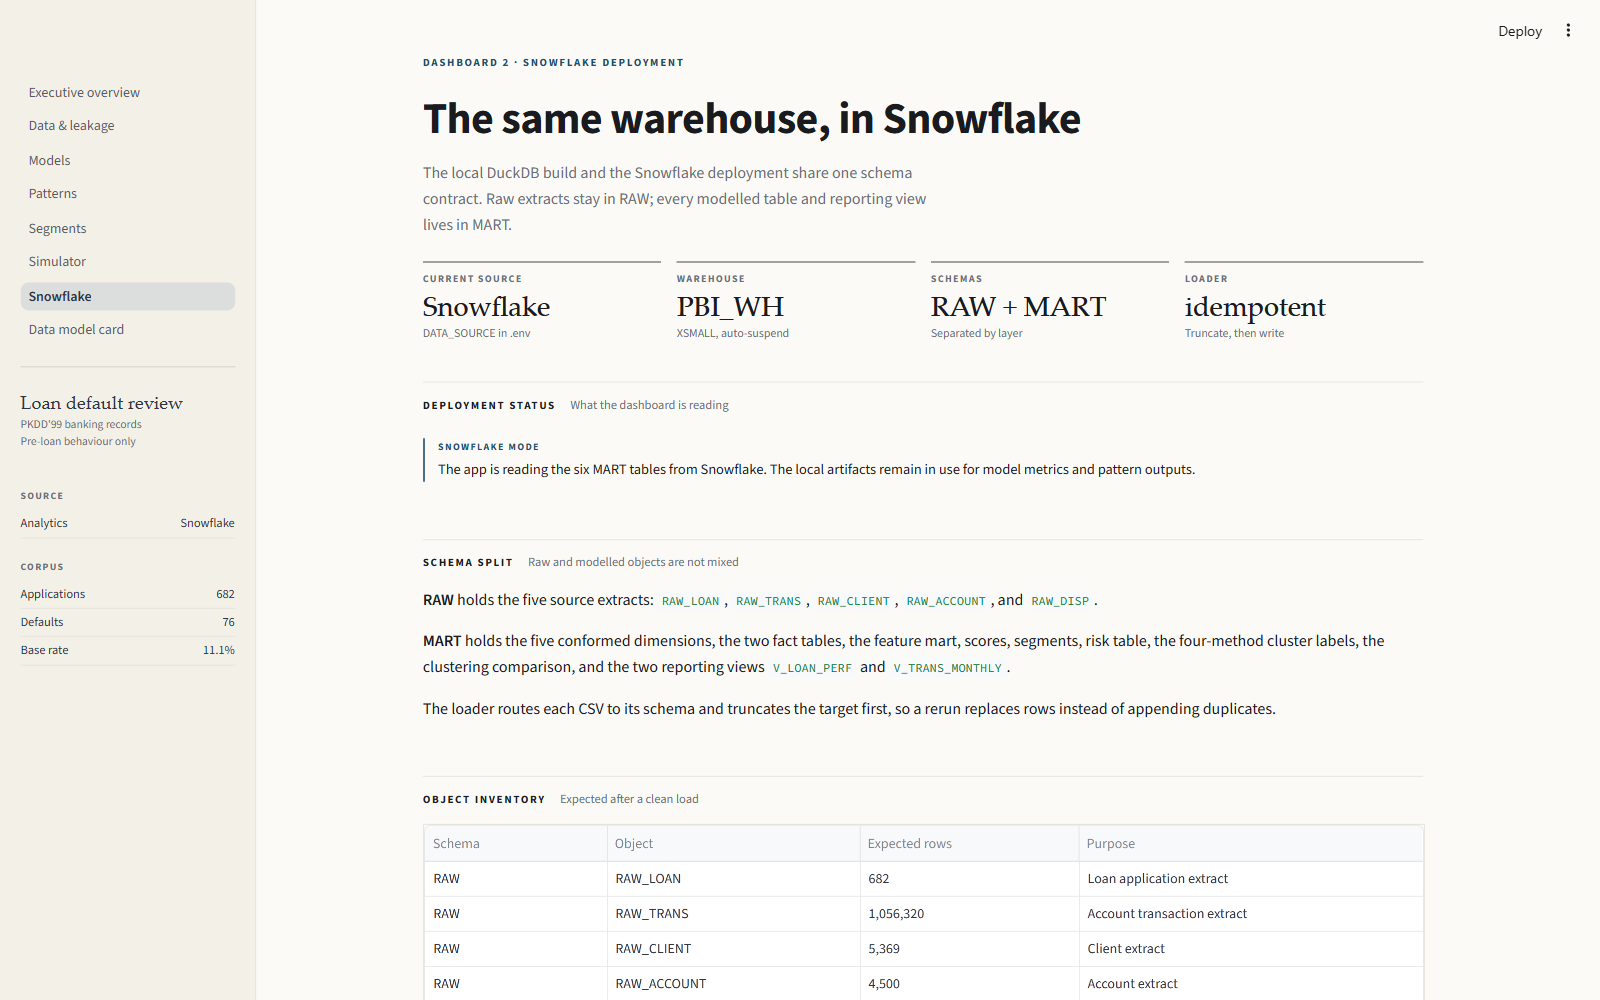
\includegraphics[width=0.92\textwidth]{figures/27_dashboard_snowflake.png}
    \caption{Streamlit dashboard: Snowflake deployment page}
    \label{fig:snowflake_page}
\end{figure}
